\section{Grad-CAM}
Grad-CAM \cite{selvaraju2017grad} (Gradient-weighted Class Activation Mapping) is a white box method. It requires insight into the convolutional neural network architecture and is therefore only applicable on convolutional neural networks. The method generates a heat map similar to RISE. Figure \ref{grad_cam_cat} and Figure \ref{grad_cam_dog} are outputs of Grad-CAM on an example image.
\captionsetup[figure]{font=Large,labelfont=Large}
\begin{figure}[H]
    \centering
    \begin{subfigure}{.5\textwidth}
        \centering
        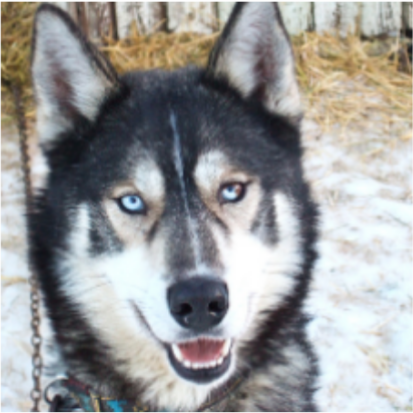
\includegraphics[width=0.95\linewidth]{images/wolf.png}
        \caption{}
    \end{subfigure}%
    \begin{subfigure}{.5\textwidth}
        \centering
        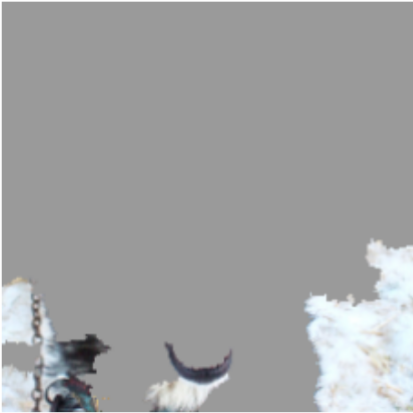
\includegraphics[width=0.95\linewidth]{images/wolf2.png}
        \caption{}
    \end{subfigure}
    \caption{Grad-CAM applied on an image with multiple valid classes. Explanation for class "cat" \cite{selvaraju2017grad}.}
    \label{grad_cam_cat}
\end{figure}

\begin{figure}[H]
    \centering
    \begin{subfigure}{.5\textwidth}
        \centering
        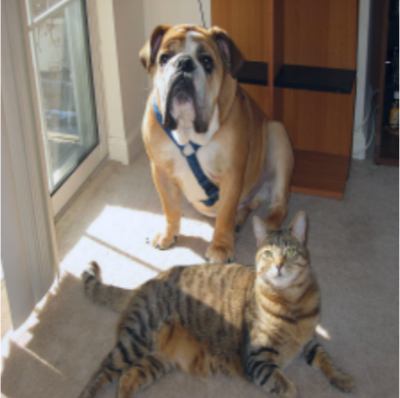
\includegraphics[width=0.7\linewidth]{chapters/02_methods/images/grad-cam-original.png}
        \caption{Original image}
    \end{subfigure}\hfill%
    \begin{subfigure}{.5\textwidth}
        \centering
        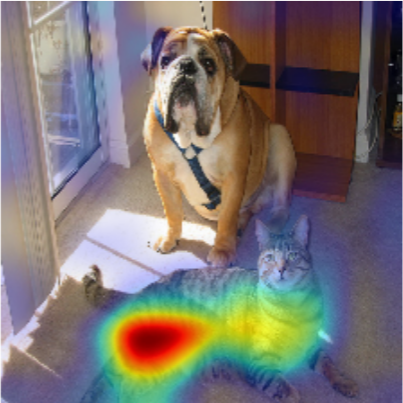
\includegraphics[width=0.7\linewidth]{chapters/02_methods/images/grad-cam-cat.png}
        \caption{Grad-CAM explanation for class "cat"}
    \end{subfigure}
    \caption{Grad-CAM applied on an image with multiple valid classes. Explanation for class "cat" \cite{selvaraju2017grad}.}
    \label{grad_cam_cat}
\end{figure}

\begin{figure}[H]
    \centering
    \begin{subfigure}{.5\textwidth}
        \centering
        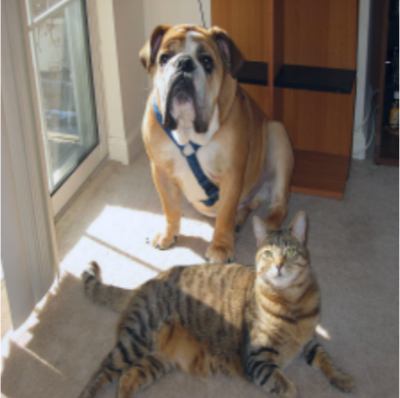
\includegraphics[width=0.7\linewidth]{chapters/02_methods/images/grad-cam-original.png}
        \caption{Original image}
    \end{subfigure}\hfill%
    \begin{subfigure}{.5\textwidth}
        \centering
        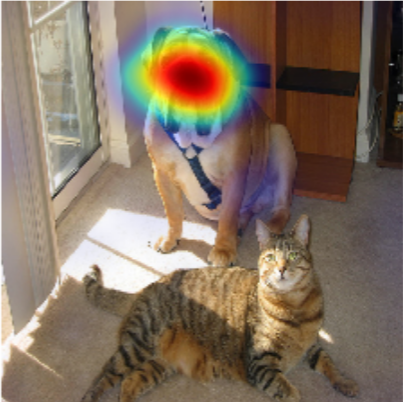
\includegraphics[width=0.7\linewidth]{chapters/02_methods/images/grad-cam-dog.png}
        \caption{Grad-CAM explanation for class "dog"}
    \end{subfigure}
    \caption{Grad-CAM applied on an image with multiple valid classes. Explanation for class "dog" \cite{selvaraju2017grad}.}
    \label{grad_cam_dog}
\end{figure}

The main parameter for this method is which convolutional layer of the neural network should be analyzed. Figure \ref{grad_cam_explanation} shows a schematic of the inner working of Grad-CAM for a layer: The feature map, i.e. the result of applying the convolution kernels on the input channel, of the specified convolutional layer is extracted. Every channel of the feature map is weighted, based on how much it influences the final output value of the network for a specific class. Finally, the weighted channels are summed up, passed through ReLU and converted to a heat map by upsampling. The ReLU is applied to remove pixels which negatively impact the class output.

\begin{figure}[H]
\centering
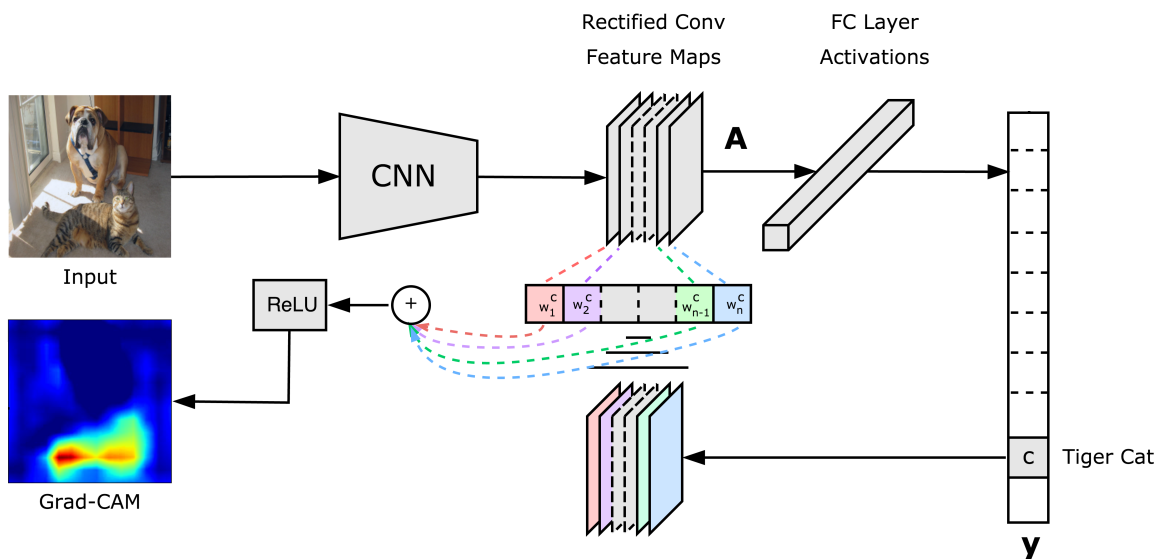
\includegraphics[width=12cm]{chapters/02_methods/images/grad-cam.png}
\caption{Grad-CAM in action: The feature map of a specific network layer is extracted, each channel weighted by the activation of the expected class, summed up and converted into a heat map.}
\label{grad_cam_explanation}
\end{figure}

